\documentclass[
  prx,
  reprint,
  superscriptaddress,
  amsmath,
  amssymb,
  aps
]{revtex4-2}

\usepackage{graphicx}
\usepackage{bm}
\usepackage{physics}
\usepackage[hidelinks]{hyperref}
\usepackage{xcolor}

\begin{document}

\title{Finite Dynamical Resource Manifolds from Non-Adiabatic Curvature and Operator Topology}

\author{Hang Hu}
\email{hang.hu@cnrc-nrc.gc.ca}
\affiliation{Digital Technologies, National Research Council of Canada, 222 College Street, Toronto, ON M5T 3J1, Canada}

\author{Hsu Kiang Ooi}
\affiliation{Digital Technologies, National Research Council of Canada, 222 College Street, Toronto, ON M5T 3J1, Canada}

\author{Anguang Hu}
\email{anguang.hu@forces.gc.ca}
\affiliation{Suffield Research Centre, Defence Research and Development Canada, PO Box 4000 Station Main, Medicine Hat, Alberta T1A 8K6, Canada}

\date{\today}

\begin{abstract}
Quantum technologies rely on entanglement, coherence, superposition, and interference as operational resources, but in realistic systems these resources compete with decoherence, control error, and measurement overhead. Here we use Entanglement--Dynamic Topology (EDT) in a restricted and falsifiable sense: EDT is said to be present only when a finite parameter window can be extracted from observables by an explicit diagnostic and shown to degrade outside that window. We implement this idea in three settings. In K$_3$C$_{60}$, EDT is identified by a nonzero momentum interval $\Delta k_{\rm EDT}$ over which paired curvature branches admit a local quadratic description below a residual threshold. In a four-qubit plaquette model, EDT is identified by an interior maximum of a combined dynamical score built from mid-time out-of-time-order correlator weight and long-time correlation, together with bounded Trotter error under approximate implementation. In NV-center AC magnetometry, EDT is identified by an interior optimum of a resource-resolved XY8 sensing proxy over pulse spacing and block count, where filter gain, coherence retention, pulse fidelity, and readout efficiency remain jointly effective. These results do not establish a universal quantum principle; rather, they provide a reproducible diagnostic workflow for detecting finite, quantitatively identifiable operating windows in distinct quantum systems.
\end{abstract}

\maketitle

\section{Introduction}

Quantum computation, sensing, and materials design depend on the controlled use of quantum resources, including entanglement, coherence, superposition, and interference~\cite{NielsenChuang,Horodecki2009,Streltsov2017}. These resources are often discussed as quantities to be increased, enlarged, or protected globally, leading naturally to strategies that explore increasingly large Hilbert spaces~\cite{Preskill2018,Arute2019}. In realistic systems, however, the same mechanisms that generate quantum resources can also degrade their usefulness through decoherence, uncontrolled spreading, pulse errors, and measurement overhead~\cite{Eisert2010,Altman2015}. This motivates a finite-regime view: useful dynamics may occur in intermediate regions where resources are generated strongly enough to be observable but remain structured enough to be controlled.

In this work, EDT is used in an operational rather than universal sense. We say that an EDT regime is present only when a finite parameter window can be extracted from observables by an explicit diagnostic and when the diagnostic degrades outside that window. Figure~\ref{fig:edt_concept} is therefore a heuristic organizing picture. The evidence-bearing claims are confined to three quantitative diagnostics: the residual-based curvature window in K$_3$C$_{60}$, the score-defined dynamical window in a four-qubit plaquette model, and the resource-resolved optimum in the modeled NV--XY8 sensing landscape.

This restricted definition deliberately avoids treating EDT as a new microscopic force or a new resource type. Instead, EDT is a diagnostic label for finite windows in which existing resources are simultaneously generated, structured, and dynamically stable. In materials, the relevant observable is the curvature of electronic energies with respect to normal-mode coordinates. In minimal quantum dynamics, the relevant observables are operator-spreading and correlation-retention metrics. In sensing, the relevant observables are filter gain, coherence retention, pulse fidelity, and readout efficiency. The central result is therefore not a claim of universality, but a reproducible workflow for asking whether a finite, measurable resource window exists in a given system.

\section{Operational definition of the EDT regime}

Let $x$ denote a control coordinate. Depending on the setting, $x$ may be a crystal momentum $k$, a normal-mode displacement $Q$, a loop coupling $\lambda$, a circuit depth, a pulse spacing $\tau$, or a pulse number $N_\pi$. We define an EDT window as a finite region $\Delta x_{\rm EDT}$ satisfying diagnostic conditions of the form
\begin{equation}
\Delta x_{\rm EDT}
=
\left\{x:
S_{\rm pair}(x)>S_{\rm pair}^{(0)},\;
R_{\rm fit}(x)<R_{\rm fit}^{(0)},\;
S_{\rm dyn}(x)>S_{\rm dyn}^{(0)}
\right\},
\label{eq:edt_window_general}
\end{equation}
where $S_{\rm pair}$ measures the compatibility of paired branches or paired response channels, $R_{\rm fit}$ measures the residual of the local reduced description, and $S_{\rm dyn}$ measures whether the corresponding dynamics remain operationally useful. In settings where only a subset of these quantities is meaningful, the diagnostic is specialized but the logic is unchanged: an EDT claim requires an explicit observable, a finite extracted window, and degradation outside that window.

For comparison across systems we use a normalized score
\begin{equation}
S_{\rm EDT}(x)
=
S_{\rm pair}(x)\,S_{\rm fit}(x)\,S_{\rm dyn}(x)\,S_{\rm robust}(x),
\label{eq:sedt_general}
\end{equation}
where $S_{\rm fit}$ is a monotonic function of the residual, for example $S_{\rm fit}=\exp[-R_{\rm fit}/R_0]$, and $S_{\rm robust}$ quantifies stability under threshold changes, parameter perturbations, or approximate implementation. Equation~\eqref{eq:sedt_general} is not intended as a universal order parameter. It is a bookkeeping device that makes the EDT diagnostic falsifiable: if no finite window survives the stated thresholds and robustness checks, EDT is not identified for that dataset or model.

\section{Non-adiabatic curvature as a material diagnostic}

The material diagnostic begins from the dependence of electronic energies on normal-mode coordinates. For band $n$ and mode coordinate $Q_\alpha$, we define the curvature
\begin{equation}
\kappa_{n\alpha}(k)
=
\frac{\partial^2 E_n(k,Q_\alpha)}{\partial Q_\alpha^2},
\label{eq:kappa_definition}
\end{equation}
which quantifies the second-order electronic response to lattice motion. This curvature is closely related to non-adiabatic mixing near degeneracies and avoided crossings, where the electronic basis changes rapidly with nuclear coordinates~\cite{BornOppenheimer1927,Mead1979,Yarkony1996}. The associated non-adiabatic coupling matrix elements
\begin{equation}
A^{(\alpha)}_{mn}=\langle m|\partial_{Q_\alpha}|n\rangle
\label{eq:nact}
\end{equation}
define a Berry-like connection whose curvature encodes the geometric structure of the coupled electronic manifold~\cite{Berry1984,Xiao2010}.

For a candidate momentum interval centered at $k_0$, we fit paired curvature branches to a local quadratic form
\begin{equation}
\kappa_\pm(k)=a_\pm(k-k_0)^2+b_\pm+\epsilon_\pm(k),
\label{eq:quad_fit}
\end{equation}
where $\epsilon_\pm(k)$ are residuals. We define the normalized quadratic residual as
\begin{equation}
R_{\rm quad}
=
\frac{
\left[\sum_k |\epsilon_+(k)|^2+|\epsilon_-(k)|^2\right]^{1/2}
}{
\left[\sum_k |\kappa_+(k)|^2+|\kappa_-(k)|^2\right]^{1/2}
}.
\label{eq:rquad}
\end{equation}
The curvature EDT window is the largest contiguous interval satisfying
\begin{equation}
\Delta k_{\rm EDT}
=
\max_{\Delta k}\left\{\Delta k:R_{\rm quad}(\Delta k)<R_{\rm th}\right\}.
\label{eq:delta_k_edt}
\end{equation}
The threshold $R_{\rm th}$ and its sensitivity are reported with the figure-generation script and in the Supplementary Information. A finite $\Delta k_{\rm EDT}$ indicates that the paired curvature response admits a stable reduced description over a nonzero interval; failure to satisfy Eq.~\eqref{eq:delta_k_edt} means that EDT is not identified by this diagnostic.

\section{Curvature-defined EDT window in K$_3$C$_{60}$}

K$_3$C$_{60}$ provides a physically motivated test case because fulleride superconductors combine narrow electronic bands, molecular vibrational modes, and strong correlation effects~\cite{Gunnarsson1997,Capone2009}. Figure~\ref{fig:k3c60_edt} applies the residual-threshold diagnostic of Eqs.~\eqref{eq:quad_fit}--\eqref{eq:delta_k_edt} to curvature-resolved band data. The analysis identifies paired curvature branches near a crossing and extracts a nonzero momentum interval $\Delta k_{\rm EDT}$ over which both branches admit local quadratic fits below the stated residual tolerance.

The claim made here is deliberately narrow. We do not claim that this window alone determines superconducting pairing, transition temperature, or device-level performance. Rather, K$_3$C$_{60}$ is used to demonstrate that the EDT diagnostic can be applied to a real electronic-structure observable and can return a finite, quantitatively defined window. The physical interpretation is that non-adiabatic curvature is not uniformly distributed across momentum space, but can concentrate into locally organized regions where a reduced paired description is valid.

To test whether the curvature diagnostic produces false positives, the same residual-threshold workflow should be applied to control datasets. A weak-curvature control should fail the pairing-amplitude criterion, while an irregular avoided-crossing control can exhibit large curvature but fail the quadratic residual criterion. These controls distinguish finite curvature organization from both weak response and uncontrolled curvature variation. In the present manuscript, the main K$_3$C$_{60}$ result is therefore a positive diagnostic example; broader material generality requires additional systems and explicit failure cases.

\section{Minimal plaquette model of finite EDT dynamics}

The plaquette model is not intended as a material-specific effective Hamiltonian for K$_3$C$_{60}$. Instead, it is a minimal dynamical model that isolates the same diagnostic structure: local interactions, a loop-induced nonlocal term, and a finite control window in which operator spreading and correlation persistence coexist. We consider the four-qubit Hamiltonian
\begin{equation}
H
=
J\sum_{\langle i,j\rangle}Z_iZ_j
+h_x\sum_i X_i
+\lambda Z_0Z_1Z_2Z_3,
\label{eq:plaquette_hamiltonian}
\end{equation}
where $J$ controls local interactions, $h_x$ drives local rotations, and $\lambda$ controls the loop term. The plaquette operator is a minimal representation of a nonlocal loop constraint. It allows one to test whether useful dynamics occur at maximal coupling or instead at an intermediate value where spreading and memory coexist.

Operator spreading is measured using an out-of-time-order correlator (OTOC)
\begin{equation}
F(t)=\langle W^\dagger(t)V^\dagger W(t)V\rangle,
\label{eq:otoc}
\end{equation}
with $W(t)=e^{iHt}We^{-iHt}$. Correlation persistence is measured by a long-time loop or two-point correlation $C_\infty$. In the implementation used here, the dynamical EDT score is written in the conservative product form
\begin{equation}
S_{\rm EDT}(\lambda)
=
\widetilde{C}_{\rm mid}(\lambda)\,
\widetilde{C}_{\infty}(\lambda),
\label{eq:plaquette_score}
\end{equation}
where $\widetilde{C}_{\rm mid}$ is a normalized mid-time OTOC-derived spreading metric and $\widetilde{C}_{\infty}$ is a normalized long-time correlation metric. This choice makes the finite-window criterion explicit: the score is small when spreading is too weak and also small when spreading destroys persistent correlations.

Figures~\ref{fig:fig3_edt_regime} and~\ref{fig:si_4q_plaquette_trotter} show that the score develops an interior maximum at $\lambda^\star$. Small $\lambda$ produces weak operator spreading; intermediate $\lambda$ produces structured spreading together with retained long-time correlation; large $\lambda$ drives an overstructured or overdriven regime in which the joint score decreases. The relevant claim is therefore that the plaquette model exhibits a finite EDT-like operating window under the stated score and parameter scan, not that all loop-induced many-body dynamics generically exhibit EDT.

\section{Trotterized implementation and robustness}

To assess implementation robustness, time evolution under Eq.~\eqref{eq:plaquette_hamiltonian} is approximated using first-order Trotterization~\cite{Trotter1959,Suzuki1990,Lloyd1996,Childs2019}. The circuit decomposition separates the $Z_iZ_j$ interactions, transverse-field rotations, and the four-body plaquette phase. Approximation quality is quantified by comparing exact and Trotterized observables, including the OTOC, long-time correlation, and the peak location $\lambda^\star$.

The purpose of this analysis is not to claim immediate hardware advantage. It is to test whether the finite diagnostic window is destroyed by approximate implementation. The Trotter results show that the extracted optimum remains stable over a finite range of step counts and that observable errors remain bounded in the regime used to identify $S_{\rm EDT}$. This supports the interpretation of the plaquette result as an implementable finite-regime diagnostic rather than a purely analytic artifact.

\section{Finite resource window in NV--XY8 sensing}

The NV-center example is treated as an experimentally motivated sensing case study, not as a direct experimental proof of the same microscopic electron--phonon mechanism. In NV-center AC magnetometry, XY8 dynamical decoupling acts as a tunable filter: the pulse spacing $\tau$ selects the target frequency, while the pulse number $N_\pi$ controls selectivity and accumulation time~\cite{Degen2017,Barry2020,Casola2018}. Increasing control strength can improve filter gain, but it also increases exposure to decoherence, pulse infidelity, and readout overhead.

The resource vector used in the sensing model is
\begin{equation}
\mathcal{R}
=
\{R_{\rm ph},\,C,\,T_2(N_\pi),\,\chi(\omega),\,\mathrm{duty}\},
\label{eq:nv_resource_vector}
\end{equation}
where $R_{\rm ph}$ is the detected photon rate, $C$ is the fluorescence contrast, $T_2(N_\pi)$ is the coherence time under dynamical decoupling, $\chi(\omega)$ is the filter response, and $\mathrm{duty}$ accounts for initialization and readout overhead. A representative sensitivity proxy scales as
\begin{equation}
\eta_{\rm AC}(\omega)
\propto
\frac{1}{\chi(\omega)C\sqrt{R_{\rm ph}T_2(N_\pi)}}\,f_{\rm duty}.
\label{eq:nv_sensitivity}
\end{equation}
Sweeps over $(\tau,N_\pi)$ identify a finite optimum where filter gain, coherence retention, pulse fidelity, and readout efficiency remain jointly effective.

Figure~\ref{fig:fig5_nvdemo} therefore supports a control-space version of the EDT diagnostic: for the modeled XY8 scenarios studied here, EDT corresponds to a finite control window in $(\tau,N_\pi)$, not to a universal sensing principle. This distinction is important because the NV model demonstrates resource balancing in an established sensing platform, whereas the K$_3$C$_{60}$ curvature diagnostic addresses a microscopic material observable.

\section{Discussion}

The present results support EDT as a reproducible diagnostic for finite operating windows in the three systems studied here. In K$_3$C$_{60}$, the diagnostic is a residual-defined curvature window; in the plaquette model, it is an interior optimum of an OTOC--correlation score; and in NV--XY8 sensing, it is a finite control region where filter gain, coherence, pulse fidelity, and readout remain jointly effective. These results do not by themselves establish universality. Rather, they define a falsifiable workflow: an EDT claim requires an explicit observable, a finite extracted window, degradation outside that window, and robustness against threshold or parameter variation.

This finite-regime view complements existing perspectives on quantum resources. It does not replace entanglement theory, coherence theory, tensor-network representations, or electron--phonon theory~\cite{Horodecki2009,Streltsov2017,Verstraete2008,Orus2014,BardeenPines1955,BCS1957}. Instead, it asks a different operational question: given a realistic system with competing resource-generating and resource-degrading mechanisms, is there a finite parameter window where useful structure is jointly optimized? The answer is supplied by diagnostics rather than by terminology.

Several limitations should be emphasized. First, the K$_3$C$_{60}$ analysis identifies a curvature-based diagnostic window, but it does not alone prove that this window controls superconducting pairing or device-level performance. Second, the plaquette Hamiltonian is a minimal model of finite-window dynamics, not a quantitatively fitted Hamiltonian for K$_3$C$_{60}$. Third, the NV--XY8 analysis is a resource-resolved modeling study based on established sensing ingredients, not a new experimental demonstration. These limitations make the EDT proposal falsifiable: broader claims require additional materials, explicit failure cases, and consistent threshold-based diagnostics.

\section{Methods}

\subsection{Electronic-structure and curvature analysis}

The K$_3$C$_{60}$ analysis uses curvature-resolved band data generated by the accompanying script listed in the asset manifest. For a symmetric displacement $\pm\Delta Q_\alpha$, the curvature may be computed by the finite-difference expression
\begin{equation}
\kappa_{n\alpha}(k)
\approx
\frac{E_n(k,+\Delta Q_\alpha)-2E_n(k,0)+E_n(k,-\Delta Q_\alpha)}{(\Delta Q_\alpha)^2}.
\label{eq:finite_difference_curvature}
\end{equation}
The paired branches are selected near the crossing region and fitted using Eq.~\eqref{eq:quad_fit}. The extracted $\Delta k_{\rm EDT}$ is reported only for intervals satisfying the residual criterion in Eq.~\eqref{eq:delta_k_edt}. Threshold sensitivity and additional control tests should be reported in the Supplementary Information.

\subsection{Plaquette dynamics}

The plaquette Hamiltonian in Eq.~\eqref{eq:plaquette_hamiltonian} is simulated by exact diagonalization for four qubits. OTOCs are computed using Eq.~\eqref{eq:otoc}, and the dynamical EDT score is computed using Eq.~\eqref{eq:plaquette_score}. The loop strength $\lambda$ and transverse field $h_x$ are swept to identify $\lambda^\star$, the interior maximum of $S_{\rm EDT}(\lambda)$.

\subsection{Trotter circuit simulation}

First-order Trotterized dynamics approximate $e^{-iHt}$ by products of exponentials of the local $Z_iZ_j$ terms, transverse-field $X_i$ terms, and the four-body plaquette term. The approximation is evaluated by comparing exact and Trotterized values of OTOCs, long-time correlations, $S_{\rm EDT}$, and the fitted optimum $\lambda^\star$. The Supplementary Information gives the circuit decomposition for the two-body and four-body phase rotations.

\subsection{NV--XY8 resource model}

The NV sensing model maps control variables $(\tau,N_\pi)$ and experimental parameters to resource factors in Eq.~\eqref{eq:nv_resource_vector}. The XY8 filter response is peaked near $\omega\simeq\pi/\tau$, while increasing $N_\pi$ changes selectivity, total evolution time, accumulated pulse error, and overhead. The reported optimum is the minimum of the sensitivity proxy in Eq.~\eqref{eq:nv_sensitivity}, or equivalently the maximum of its inverse resource score.

\section*{Data availability}

The data supporting the figures and quantitative conclusions of this work are provided with the accompanying repository assets, including the K$_3$C$_{60}$ AGR dataset, processed curvature outputs, plaquette-model simulation outputs, NV-resource model inputs, and scripts required to regenerate the figures.

\section*{Code availability}

The analysis code used to compute EDT diagnostics, curvature windows, plaquette dynamics, Trotterized circuits, NV--XY8 sensing scores, and figure generation is provided with the accompanying repository assets.

\section*{Competing interests}

The authors declare no competing interests.

\begin{figure*}[t]
\centering
\includegraphics[width=0.92\linewidth]{figs/fig1_edt_framework_camera_ready.pdf}
\caption{\textbf{Operational picture of EDT as a finite-window diagnostic.}
(A) Near degeneracies and avoided crossings provide locations where non-adiabatic curvature can become enhanced. (B) A reduced, structured region is embedded within the full Hilbert space. (C) The structure can motivate symmetry-adapted or circuit-level representations. (D) The diagnostic compares unstructured parameter exploration with finite-window operation. (E) Sampling or control strategies are restricted to task-relevant sectors. (F) In sensing platforms, finite control windows arise when selectivity, coherence, pulse fidelity, and readout remain jointly effective. This figure is heuristic; the evidence-bearing diagnostics are shown in Figs.~\ref{fig:k3c60_edt}--\ref{fig:fig5_nvdemo}.}
\label{fig:edt_concept}
\end{figure*}

\begin{figure*}[t]
\centering
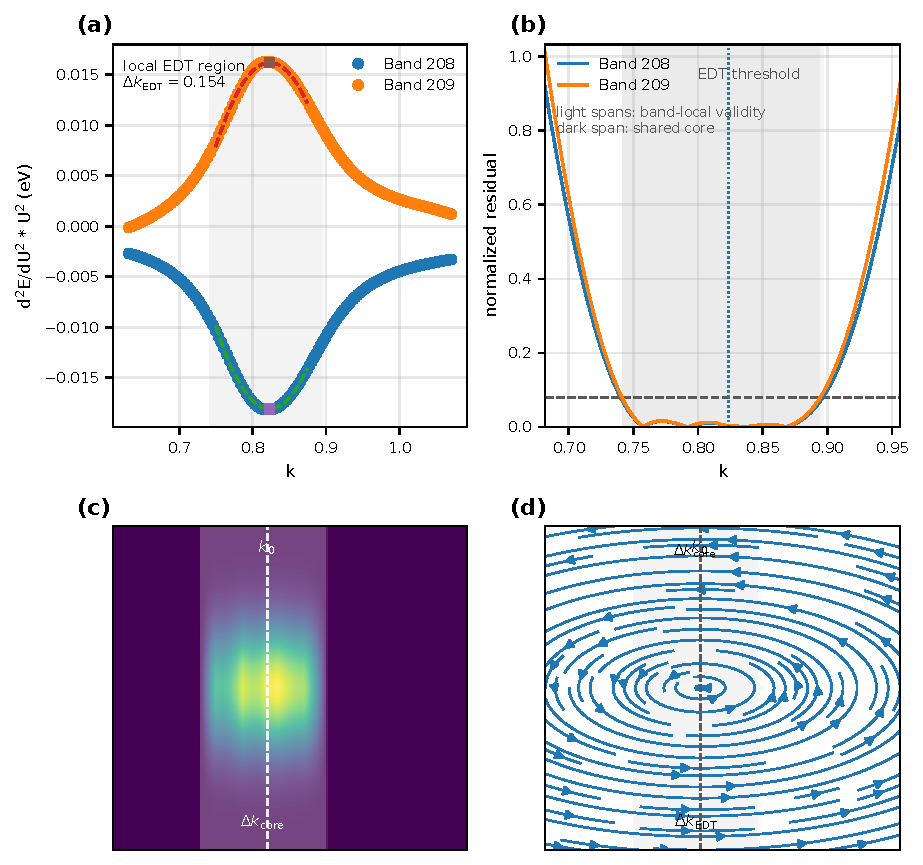
\includegraphics[width=0.92\linewidth]{fig_S7_NACT_K3C60_EDT_localfit_datamap.pdf}
\caption{\textbf{Residual-defined curvature window in K$_3$C$_{60}$.}
(a) Curvature of band energies near a crossing, showing localized second-order response. (b) Residual analysis defining the validity of local quadratic fits for paired curvature branches. (c) Local quadratic structure characterized by an intrinsic scale $k_0$ and a core region $\Delta k_{\rm core}$. (d) Extracted EDT window $\Delta k_{\rm EDT}$, defined as the largest momentum interval over which paired curvature branches satisfy the residual threshold. The claim supported by this figure is the existence of a finite curvature-diagnostic window for the dataset analyzed here.}
\label{fig:k3c60_edt}
\end{figure*}

\begin{figure*}[t]
\centering
\includegraphics[width=0.98\linewidth]{figs/figure3_edt_regime_panel.pdf}
\caption{\textbf{Finite EDT-like regime from loop-controlled plaquette dynamics.}
(a) OTOC map $C_{\rm OTOC}(t,\lambda)$ showing loop-induced operator spreading. (b) Comparison of OTOC summaries with the long-time correlator $C_\infty$. Operator spreading increases with loop strength, while $C_\infty$ decreases at large $\lambda$; their overlap defines a finite operating window. (c) OTOC time-structure metrics. (d) Combined EDT score, showing an interior maximum. (e) Classification into local, finite-window, and overdriven regimes. (f) Dependence of the optimal loop strength $\lambda^\star$ on $h_x$.}
\label{fig:fig3_edt_regime}
\end{figure*}

\begin{figure*}[t]
\centering
\includegraphics[width=0.80\linewidth]{figs/demo_edt_gyro_trotter_4q_plaquette_otoc.pdf}
\caption{\textbf{Trotterized implementation and robustness of the plaquette diagnostic.}
(a) Optimal loop strength $\lambda^\star$ under variation of the transverse field $h_x$. (b) Peak EDT score $S^\star_{\rm EDT}$, showing non-monotonic dependence on $h_x$. (c) Circuit depth and gate count versus evolution time for the first-order Trotter implementation. (d) Observable and OTOC errors versus time. (e) Stability of $\lambda^\star$ versus Trotter budget. (f) Peak EDT score versus Trotter budget. The purpose of this figure is to test whether the finite diagnostic window survives approximate implementation.}
\label{fig:si_4q_plaquette_trotter}
\end{figure*}

\begin{figure*}[t]
\centering
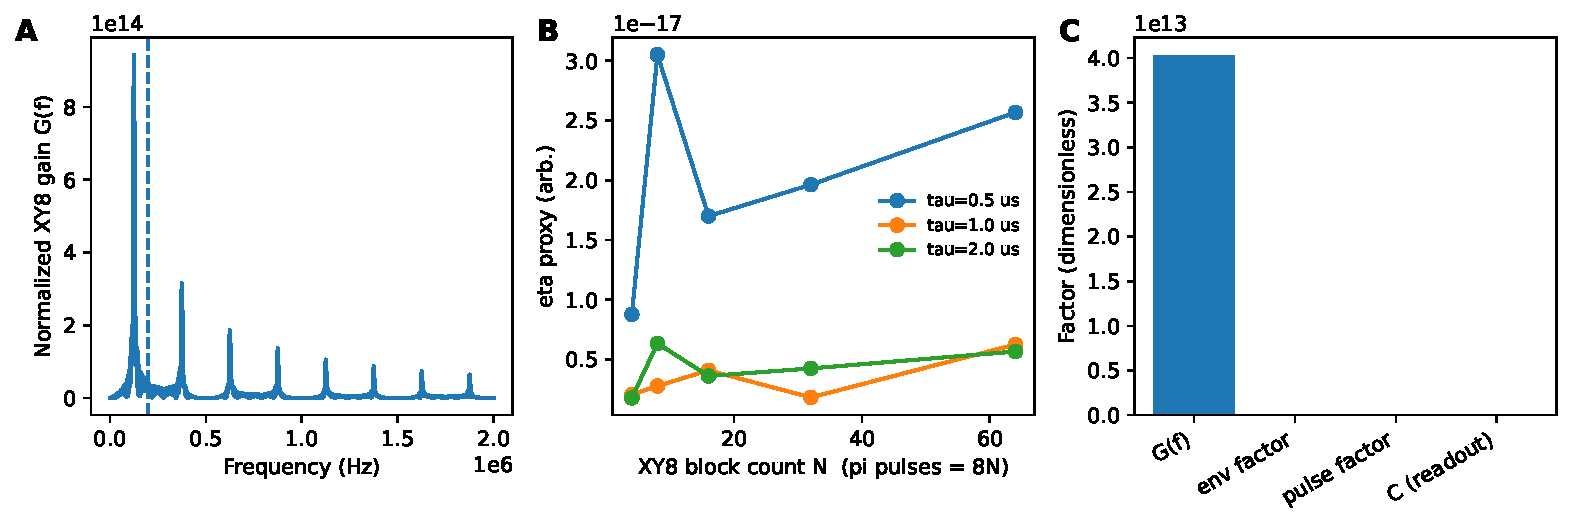
\includegraphics[width=0.90\linewidth]{figs/fig_xy8_qre_nv.pdf}
\caption{\textbf{Finite resource window in modeled NV-center XY8 sensing.}
(A) XY8 filter response $G(f)$ showing frequency-selective amplification. (B) Sensitivity proxy as a function of pulse number $N_\pi$ and spacing $\tau$, showing a finite optimum. (C) Decomposition into filter gain, environmental coherence, pulse fidelity, and readout contrast. The NV analysis is an experimentally motivated control-space case study, not a new experimental demonstration of a universal EDT principle.}
\label{fig:fig5_nvdemo}
\end{figure*}

\bibliographystyle{apsrev4-2}
\bibliography{references}

\end{document}
